%% uctest.tex 11/3/94
%% Copyright (C) 1988-2004 Daniel Gildea, BBF, Ethan Munson.
%
% This work may be distributed and/or modified under the
% conditions of the LaTeX Project Public License, either version 1.3
% of this license or (at your option) any later version.
% The latest version of this license is in
%   http://www.latex-project.org/lppl.txt
% and version 1.3 or later is part of all distributions of LaTeX
% version 2003/12/01 or later.
%
% This work has the LPPL maintenance status "maintained".
% 
% The Current Maintainer of this work is Daniel Gildea.



\documentclass[11pt]{ucthesis}
\def\dsp{\def\baselinestretch{2.0}\large\normalsize}
\dsp

\usepackage{lineno}
\modulolinenumbers[5]
\usepackage{graphicx}
\usepackage{booktabs}
\usepackage{amssymb,amsmath,nccmath}

\usepackage{cclicenses}
\usepackage{makecell}
\usepackage{lscape,array}
\newcolumntype{C}[1]{>{\centering\arraybackslash}p{#1}} 
\usepackage[thin, , thinc]{esdiff}
\usepackage{subcaption}
\usepackage{caption}
\usepackage{framed}  
\usepackage[font=small,skip=0pt]{caption}
\usepackage{url}
\usepackage{wrapfig}
\usepackage{float}
\usepackage{multirow}
\usepackage{amsmath}
\usepackage{tikz}
\usepackage{tikz-3dplot}
\usepackage{mathrsfs}
\usetikzlibrary{arrows}
\newcommand{\AxisRotatorA}[1][rotate=0]{%
	\tikz [x=0.25cm,y=0.60cm,line width=.2ex,-stealth,#1] \draw (0,0) arc (-150:150:1 and 1);%
}
\newcommand{\AxisRotatorB}[1][rotate=0]{%
	\tikz [x=0.25cm,y=0.60cm,line width=.2ex,-stealth,#1] \draw (0,0) arc (150:-150:1 and 1);%
}

\usepackage{titlesec}

\titleformat{\chapter}{\normalfont\huge}{\thechapter.}{20pt}{\huge\it}
\begin{document}

% Declarations for Front Matter

\title{PID Controller Theory Applied to Unmanned Ariel Vehicles}
\author{Rick Ramirez}
\degreeyear{2020}
\degreemonth{March}
\degree{Bachelor of Science}
\chair{ }
\committeememberone{Professor }


\numberofmembers{3} %% (including chair) possible: 3, 4, 5, 6
\deanlineone{}
\deanlinetwo{}
\deanlinethree{}
\field{Physics}
\campus{Santa Cruz}

\begin{frontmatter}

\maketitle


\tableofcontents
\listoffigures
\listoftables





\end{frontmatter}

\chapter{Quadcopter Dynamics}
\vspace{-1cm}
\section*{Introduction}
Unmanned aerial vehicles (UAV) are convenient tools when manned flight is considered too risky and prove to be useful in applications ranging from military and law enforcement, to photography, journalism, and delivery services. The global demand for commercial unmanned aerial systems is predicted to have market revenues exceed \$2 billion by 2024 \cite{foster2019} and as of 2020, compact quadcopters with a diagonal measurement of less than 12cm are readily accessible to the general hobbyist and are becoming cheaper and more advanced every quarter. 

A typical quadcopter design consist of four motors attached to the ends of each arm with adjacent motors spinning in opposite directions as shown in figure \ref{fig:wizard1}. The arms are arranged in an X-configuration with the flight controller (and sometimes electronic speed controllers (ESC)) mounted to the center of the craft. Depending on the design of the frame, the battery used to power the copter is usually mounted above or below the flight controller. 

The purpose of this thesis is to build and modify an existing quadcopter design, to obtain a stable flight, to investigate the dynamics of quadcopter motion in free space, and to analyze the effects of turbulence produced by "prop-wash" (the disturbed mass of air pushed by the propeller) during a descent. The investigation of prop-wash was performed through proportional-integral-derivative (PID) controller theory using betaflight 3.4 \cite{Betaflight}, see figure \ref{fig:pidSample}. Although the use of a PID algorithm does not guarantee optimal control of the system or its stability, in practical terms, this control loop mechanism provides accurate corrections to a control function.
\newpage
\section{Quadcopter Kinematics}
\subsection{Rotation Matrices}
\begin{wrapfigure}{l}{0pt}
	\tdplotsetmaincoords{70}{30}
	\begin{tikzpicture}[tdplot_main_coords][H]
	\coordinate (O) at (0,0,0);
	\draw[->] (O) --++ (4,0,0) node [midway] {\AxisRotatorA[rotate=180]} node[below] {$x$} node[] at (2,1,0){$\phi$};
	\draw[->] (O) --++ (0,-4,0) node [midway] {\AxisRotatorA} node[below] {$y$} node[] at (0,-2,1){$\theta$};
	\draw[->] (O) --++ (0,0,4) node [midway] {\AxisRotatorA[rotate=90]} node[right] {$z$} node[] at (1,0,2){$\psi$};
	\end{tikzpicture}
	\caption{Yaw, pitch, and roll angles}
\end{wrapfigure}
In aviation, rotations about the three orthogonal axes $\{x,y,z\}$ correspond to the following rotation matrices and terminology. $\bold{R}(\phi,\theta,\psi) = R_x(\phi)R_y(\theta)R_z(\psi)$, see Eq \ref{eq:1}, where "roll" is a counterclockwise (CCW) rotation of $\phi$ about the $x$-axis, "pitch" is a CCW rotation of $\theta$ about the $y$-axis, and "yaw" is a CCW rotation of $\psi$ about the $z$-axis.
\begin{equation}\label{eq:1}
\hspace*{-2cm} % Adjust horizontal spacing
\begin{matrix}
R_z(\psi)=\begin{bmatrix}
\cos\psi & -\sin\psi & 0\\
\sin\psi & \cos\psi & 0\\
0 & 0 & 1
\end{bmatrix} 
&
R_y(\theta)=\begin{bmatrix}
\cos\theta & 0 & \sin\theta\\
0 & 1 & 0\\
-\sin\theta & 0 & \cos\theta
\end{bmatrix} 
&
R_x(\phi)=\begin{bmatrix}
0 & \cos\phi & -\sin\phi\\
0 & \sin\phi & \cos\phi\\
-\sin\theta & 0 & \cos\theta
\end{bmatrix}
\end{matrix}
\end{equation}
It is important to note that under this convention, the transformation sequence of $\bold{R}(\psi,\theta,\phi)$ first performs the yaw, then the pitch, and finally the roll. A change in the sequence will produce a different rotation matrix which will cause errors when calculating for corrections. This is especially important when considering stabilization effects through PID corrections because without the use of quaternion methods, the PID controller is reliant on the Euler angle calculations having unique solutions. If the orientation of the flight controller doesn't match the rotation matrix, the copter is likely to spiral out of control when receiving input from the transmitter. Another issue that could manifest from alternating rotation order is the location of singularities of the axes which will lead to gimbal lock (the loss of a degree of freedom in the gyro). For the $(\psi,\theta,\phi)$ convention, a singularity occurs when the pitch axis is rotated by $\theta = \pm \:90^\circ$, in which case $\psi$ and $\phi$ are aligned. This will cause yaw and roll movements to produce the same results. However, using $(\theta,\psi,\phi)$ would produce a singularity at $\psi = \pm \:90^\circ$. The complete 3D matrix gives Eq \ref{eq:2} \cite{fantoni2002non}
\begin{equation}\label{eq:2}
\hspace*{-1cm} % Adjust horizontal spacing
\bold{R}(\phi,\theta,\psi) = \begin{bmatrix}
\cos\psi\cos\theta & \cos\psi\sin\theta\sin\phi - \sin\psi\cos\phi & \cos\psi\sin\theta\cos\phi + \sin\psi\sin\phi\\
\sin\psi\cos\theta & \sin\psi\sin\theta\sin\phi + \cos\psi\cos\phi & \sin\psi\sin\theta\cos\phi - \cos\psi\sin\phi\\
-\sin\theta & \cos\theta\sin\phi & \cos\theta\sin\phi
\end{bmatrix}
\end{equation}

\subsection{Equations of Motion}
In the inertial frame, the copter has 6 degrees of freedom, $(x,y,z,\psi,\theta,\phi)$. From Figure \ref{fig:Quadcopter}, $\mathscr{B} = \{B_1,B_2,B_3\}$ is the body fixed frame, $\mathscr{E} = \{E_x,E_y,E_z\}$ is the inertial frame fixed with respect to the earth. The vector $\xi$ corresponds to the position $(x,y,z)$ of the center of mass with respect to the inertial frame  $\mathscr{E}$, and the vector $\eta$ consists of the Euler angles $(\psi,\theta,\phi)$ representing the orientation of the copter as shown in Eq. \ref{eq:coordinates} \cite{garcia2006modelling}.

\begin{equation}\label{eq:coordinates}
\xi = [x,y,z]^T  \qquad \text{and} \qquad \eta = [\psi,\theta,\phi]^T \quad\footnote{Superscript $T$ is the transpose of the matrix.}
\end{equation}
The coordinates of the body frame from the inertial frame is given by Eq \ref{eq:2}; that is, $\mathscr{B} =\bold{R}\mathscr{E} $. 
\newpage

\begin{figure}
\tdplotsetmaincoords{70}{110}
\begin{center}
	\begin{tikzpicture}[tdplot_main_coords][!h]
	\draw (-8,0,0) -- (8,0,0) ;
	\draw (0,-5,0) -- (0,5,0);
	\draw[dashed,<->] (0,0,-3) -- (0,0,3);
	\draw (-8,0,0) ellipse (1cm and 0.5cm);
	\draw (8,0,0) ellipse (1cm and 0.5cm);
	\draw (0,5,0) ellipse (1cm and 0.5cm);
	\draw (0,-5,0) ellipse (1cm and 0.5cm);
	\draw (-8,0,0) node [red] {\AxisRotatorB[rotate=-90]};
	\draw (8,0,0.1) node [red] {\AxisRotatorB[rotate=-90]};
	\draw (0,5,0) node [blue] {\AxisRotatorA[rotate=-90]};
	\draw (0,-5,0) node [blue] {\AxisRotatorA[rotate=-90]};
	% Force vectors
	\draw[thick,->] (-8,0,1) -- (-8,0,2) node[above] {$f_1$};
	\draw[thick,->] (8,0,1) -- (8,0,2) node[above] {$f_3$};
	\draw[thick,->] (0,5,1) -- (0,5,2) node[above] {$f_4$};
	\draw[thick,->] (0,-5,1) -- (0,-5,2) node[above] {$f_2$};
	% Motors
	\draw(-9.5,1,0) -- (-9.5,1,0) node {$M1$};
	\draw(0,-6.5,0) -- (0,-6.5,0) node {$M2$};
	\draw(9,-1.5,0) -- (9,-1.5,0) node {$M3$};
	\draw(0,6.5,0) -- (0,6.5,0) node {$M4$};
	% Net thrust & gravity 
	\draw (0,0,-2) -- (0,0,-3) node[below] {$mg$};
	\draw[thick,->] (0,0,2) -- (0,0,3) node[above] {$U_1$};
	% Body frame
	\node[] at (0.7,1,2) {$\mathscr{B}$};
	\draw[line width=0.5mm,->] (O) --++ (-2,0,0) node[below,right] {$B_{1}$};
	\draw[line width=0.5mm,,->] (O) --++ (0,1,0) node[below] {$B_{2}$};
	\draw[line width=0.5mm,,->] (O) --++ (0,0,1) node[right] {$B_{3}$};
	% Reference frame
	\node at (15.7,3,0) {$\mathscr{E}$};
	\node[] at (10,2.25,0) {$\xi$};
	\draw[dashed] (0,0,0) --++ (15,3,0);
	\draw[line width=0.5mm,->] (15,3,0) --++ (-2,0,0) node[below,right] {$E_{x}$};
	\draw[line width=0.5mm,->] (15,3,0) --++ (0,1,0) node[below] {$E_{y}$};
	\draw[line width=0.5mm,->] (15,3,0) --++ (0,0,1) node[left] {$E_{z}$};
	\end{tikzpicture}
	\caption{Quadcopter in an inertial frame.}
	\label{fig:Quadcopter}
\end{center}
\end{figure}
\noindent
The translational kinetic energy is
\begin{equation}
T_{trans} = \frac{m}{2}\dot{\xi}^T\dot{\xi}
\end{equation}
where $\dot{\xi}$ is the velocity of the copter in the inertial frame,
\noindent
and the rotational kinetic energy is
\begin{equation}
T_{rot} = \frac{1}{2}\nu^T\bold{I}\:\nu\qquad \text{where, }\qquad
\bold{I} = \begin{bmatrix}
I_{xx} & 0 & 0\\
0 & I_{yy} & 0\\
0 & 0 & I_{zz}
\end{bmatrix}
\end{equation}
\noindent
is the diagonal inertia matrix, with $I_{xx}=I_{yy}$, and the angular velocity in the body frame is $\nu =[p,q,r]^T$.\footnote{Note that $\omega$ is being reserved for the angular velocity of the motors while $\nu$ refers to the angular velocity of the copter itself in the body frame $\mathscr{B}$.} 
\noindent
The transformation matrix of the angular velocities from the inertial frame to the body frame is $\bold{W}_{\eta}$, and from the body frame to the inertial frame is $\bold{W}_{\eta}^{-1}$. Rotational kinematics can be obtained from the relationship between the rotation matrix and its derivative with a skew-symmetric matrix (a square matrix whose transpose equals its negative)\cite{raffo2010integral}. Because the gyro rate data is reported to the flight controller with respect to the body frame,  we require a mapping from $\nu \rightarrow \eta$. When we consider the effects of a change in each Euler angle, the effect of the rotation vector is that the first Euler angle undergoes two additional rotations, the second angle has one additional rotation, and the third angle has none as shown in Eq.\ref{eq:transform} \cite{opencoursewarekinematics}.
\begin{equation}\label{eq:transform}
\nu = R(\psi)R(\theta) \begin{bmatrix}
			0\\
			0 \\
			\dot{\psi}  
			\end{bmatrix} + 
			R(\psi)   \begin{bmatrix}
				0\\
				\dot{\theta} \\
				0  
				\end{bmatrix} + 
						\begin{bmatrix}
					\dot{\phi}\\
					0\\
					0  
					\end{bmatrix} 	=\begin{bmatrix}
					1 & 0 & -\sin\theta\\
					0 & \cos\phi & \sin\phi\cos\theta\\
					0 & -\sin\theta & \cos\phi\cos\theta
					\end{bmatrix} \begin{bmatrix}
					\dot{\phi}\\
					\dot{\theta}\\
					\dot{\psi}
					\end{bmatrix}
\end{equation}
Taking the inverse, we find the transformation to the inertial frame to be Eq.\ref{eq:skew-symmetric matrix}.
\begin{equation}\label{eq:skew-symmetric matrix}
\bold{\dot{\eta}} = \bold{W}_{\eta}^{-1} \nu \quad \rightarrow \quad
\begin{bmatrix}
\dot{\phi}\\
\dot{\theta}\\
\dot{\psi}
\end{bmatrix}  = 
\begin{bmatrix}
1 & \sin\phi\tan\theta & \cos\phi\tan\theta\\
0 & \cos\phi & -\sin\phi\\
0 & \sin\phi\sec\theta & \cos\phi\sec\theta
\end{bmatrix} 
\begin{bmatrix}
p\\
q\\
r
\end{bmatrix}
\end{equation}
The Jacobian matrix from $\nu$ to $\dot{\eta}$ is $\bold{J}(\eta) = \bold{J} = \bold{W}_{\eta}^{-1}\bold{I}\:\bold{W}_{\eta}$, which means that the rotational kinetic energy can be expressed in the inertial frame as 
\begin{equation}
T_{rot} = \frac{1}{2}\nu^T\bold{I}\:\nu = \frac{1}{2}\dot{\eta}^T \bold{J\:}\dot{\eta}
\end{equation}
Finally, the only potential energy acting on the system is that due to gravity,
\begin{equation}
U = mgz
\end{equation}
which, together with the translational and rotational terms, produces a Lagrangian of the form
\begin{equation}
L(q,\dot{q}) = T_{trans}+T_{rot}-U =  \frac{m}{2}\dot{\xi}^T\dot{\xi} + \frac{1}{2}\dot{\eta}^T \bold{J\:}\dot{\eta} - mgz
\end{equation}
where $\bold{q} = [\xi, \eta]$. As the propellers spin about their axes, air is pushed downward by the blades creating a force upward on the copter. Because, the speed of the air exiting the fan is proportional to the speed of the fan and a given volume of air passing through the fan per second is also proportional to the speed of the fan, it follows that the force, which is the mass flow rate multiplied by the velocity, is proportional the the square of the velocity of the motors. So, for each rotor $i$ there is a force in the direction of the rotor axis; and, together with the angular acceleration, a torque $T_{M_i}$ around the rotor axis,
\begin{equation}\label{eq.forces}
f_i = k\omega_i^2 ,\qquad T_{M_i} = b\omega_i^2 + I_M \dot{\omega}_i
\end{equation}
where $k$ is a lift constant and $b$ is a drag constant. In most cases, $\dot{\omega}_i$ is small enough to be omitted \cite{luukkonen2011modelling}. A thrust is created from the net force in the z-direction of the body
\begin{equation}\label{eq:thrust}
U_1 = \sum_{1=1}^{4}f_i = k\sum_{1=1}^{4}\omega_i^2
\end{equation}
and a torque 
\begin{equation}
\bold\tau_{\eta} = 
\begin{bmatrix}
\tau_\phi\\
\tau_\theta\\
\tau_\psi
\end{bmatrix} = 
\begin{bmatrix}
lk(\omega_4^2 - \omega_2^2)\\
lk(\omega_3^2 - \omega_1^2)\\
\sum_{1=1}^{4}T_{M_i}
\end{bmatrix}
\label{eq:torque}
\end{equation}
Where $l$ is the distance between the rotor and the center of mass. From Eq \ref{eq:torque}, we see that rolls are created when $\omega_4^2 - \omega_2^2 \neq 0$, pitch movement is created when $\omega_3^2 - \omega_1^2 \neq 0$, and yaw movement is created when the difference in angular velocity between sets of diagonal motors is not equal to zero; that is, $\omega_4^2 - \omega_2^2 \neq \omega_3^2 - \omega_1^2 $.

\section{Euler-Lagrange approach} 
The model for the dynamics of the quadcopter is obtained from the Euler Lagrange-equations with external generalized force \cite{castillo2005experimental, raffo2010integral, luukkonen2011modelling, garcia2006modelling}.

\begin{equation}
\left[ \frac{\bold{f}_{\xi}}{\bold{\tau}_{\eta}}\right] = \frac{d}{dt}\frac{\partial\mathcal{L}}{\partial\dot{q}} - \frac{\partial\mathcal{L}}{\partial q}
\end{equation}
where $\bold{q} = [\xi,\eta]$. $\bold{f}_{\xi} = \bold{R}\hat{\bold{f}} = \bold{R}_{e_3}U_1$ \footnote{where $\bold{e_3} $ represents $[0,0,1]^T$. When applied to $\bold{R}$, it only acts on the third column.} is the translational force applied to the quadcopter from the main control input $U_1$ as observed from the inertial frame $\mathscr{E}$. That is, from Eq. \ref{eq:thrust}, $U_1$ is the thrust in the z-direction of the body. $\bold{\tau}_{\eta}$ is the torque from Eq.\ref{eq:torque}. Because the Lagrangian does not contain cross terms between $\dot{\xi}$ and $\dot{\eta}$, the translational and rotational terms can be separated.
\begin{equation}\label{eq:translation}
m\ddot{\xi} + 
\begin{bmatrix}
0\\
0\\
mg
\end{bmatrix} = \bold{f}_{\xi}
\end{equation}

\begin{equation}\label{eq:rotation}
\bold{I}\ddot{\eta} + \dot{\bold{I}}\dot{\eta} - \frac{1}{2}\frac{\partial}{\partial\eta}(\dot{\eta}^T\bold{I}\dot{\eta}) = \tau_{\eta}
\end{equation}
From Eq \ref{eq:translation} and Eq \ref{eq:2} we find that

\vspace{-1cm}
\begin{equation}
\left\lbrace\begin{matrix}
\ddot{x} = \frac{U_1}{m} (\cos\psi\sin\theta\cos\phi + \sin\psi\sin\phi)\\
\ddot{y} = \frac{U_1}{m}(\cos\psi\sin\theta\cos\phi + \cos\psi\sin\phi) \\
\ddot{z} = \frac{U_1}{m}(\cos\theta\cos\phi) - g
\end{matrix}\right.
\end{equation}
The external angular force applied to the copter is the torque of the rotors. Looking at Eq.\ref{eq:rotation}, we find that
\vspace{-0.25cm}
\begin{equation}
\tau_{\eta} = \bold{J}\ddot{\eta} + \frac{d}{dt}({\bold{J})}\dot{\eta} -\frac{1}{2}(\dot{\eta}^t \bold{J} \dot{\eta}) = \bold{J}\ddot{\eta} + C(\eta, \dot{\eta})\dot{\eta}
\end{equation}
where $C(\eta, \dot{\eta})$ is a 3X3 matrix known as the Coriolis term which contains the gyroscopic and centrifugal terms. The form of $C(\eta, \dot{\eta})$, in this case, is quite cumbersome to work with and can be seen in Raffo et al., 2010 \cite{raffo2010integral}. To simplify things, consider the body frame of the copter. The sum of the angular acceleration $\bold{I}\bold{\dot{\nu}}$, the centripetal forces $\bold{\nu} \times (\bold{I\nu})$ and the gyroscopic force $\Gamma$ are  equal to the external torque $\tau_{\eta}$ \cite{bhosalemathematical},
\begin{equation}\label{eq:dynamicsEquations}
\begin{matrix}
\bold{I}\bold{\dot{\nu}} + \bold{\nu} \times (\bold{I\nu}) + \Gamma = \tau_{\eta}\\

\begin{bmatrix}
\dot{p}\\
\dot{q}\\
\dot{r}
\end{bmatrix} = 
\begin{bmatrix}
(I_{yy} - I_{zz})qr/I{xx}\\
(I_{zz} - I_{xx})pr/I{yy}\\
(I_{xx} - I_{yy})pq/I{zz}
\end{bmatrix}

-I_r

\begin{bmatrix}
q/I{xx}\\
-p/I_{yy}\\
0
\end{bmatrix} \omega_{\Gamma}

+ 	\begin{bmatrix}
\tau_{\phi} / I_{xx}\\
\tau_{\theta} / I_{yy}\\
\tau_{\psi} / I_{zz}
\end{bmatrix}
\end{matrix}
\end{equation}
where $\omega_{\Gamma} = \omega_1 - \omega_2 + \omega_3 - \omega_4$.
From Eq.\ref{eq:dynamicsEquations}, we find that if the UAV is designed with a well balanced load, the moment of inertia at the $x$ and $y$ axes are equal, however, in general $I_{xx} \neq I_{zz}$. Therefore, there will be interactions between $p$ and $q$ which will be registered as disturbances in the PID controller. Also, the products of the angular velocities in Eq.\ref{eq:dynamicsEquations} and the sinusoidal functions in \ref{eq:skew-symmetric matrix} produce three second order nonlinear systems. A steady state condition is achieved by setting $\phi = \theta = 0$, while allowing $\psi$ to change according to the input signal.
\clearpage
\chapter{PID Controller Theory}

In order to ensure stability of a multi-rotor unmanned aerial vehicle, its attitude, which is captured by variations of the three Euler angles ($\phi, \theta, \phi$), is required to be under feedback control. This requires the controller to handle the system in such a way that the control variable is held at its desired set point for as long as possible with minimal oscillations and minimal deviations from that set point. A system can deviate from its set point in two ways: changes in the set point itself or changes that occur to the process. These deviations can be temporary or permanent and can be either intentional or the result of external disturbances. There could also be inaccuracies present in sensors, transmitters etc. To handle the possible disturbances, the controller first determines the error, defined as the difference between the set point value $y_{sp}$ and the measured value $y_m$ \cite{wang2020pid}.
\begin{equation}
e(t) = y_{sp} - y_m
\end{equation}
Once the error is calculated, the controller can take one of three terms of it. It can take a term proportional to the error at its current state, an integral over time of the error (to account for past values), and a derivative of the error (to estimate future values). The sum of the calculated values is then fed back into the system for the next iteration. This procedure is known as a feedback loop. In textbooks, the system that the PID values are fed to is referred to as a "plant". In essence, the PID controller is attempting to minimize error over time by adjusting a control variable $U(t)$. In the case of a UAV, the plant is the flight controller, and the set point is the remote input from the pilot.
\section{Simulink}
Simulink \cite{documentationsimulation} is a MATLAB based graphical programming environment used for modeling, simulating and analyzing multidomain dynamical systems. It provides a graphical editor and customizable block libraries. The PID Controller block implements a PID controller (PID, PI, PD, P only, or I only). The block diagram is a visual representation of the control system where the blocks represent the transfer function, and arrows represent the input and output signals as shown in fig \ref{fig:pidDiagram}. The block output is a weighted sum of the input signal, the integral of the input signal, and the derivative of the input signal and the weights are the proportional, integral, and derivative gain parameters. A first-order pole filters the derivative action. Note that the simulations presented here did not use the PID block function within Simulink. Instead, individual blocks for the P, I and D terms were created, the sum of which was fed into the transfer function.

The following PID analysis simulations were created using Simulink with the "plant" (quadcopter) substituted by a transfer function $G(s)=(1+s)^{-3}$; which coincides to the form of the theoretical transfer functions used in \cite{reizenstein2017position,kugelberg2016black,aastrom2010feedback}. The transfer function of a control system is a function that theoretically models the device's output for a given input, and is typically derived from experimental data. Note that the transfer function used in this section is not the exact function used by the flight controller of the quadcopter in chapter 3 and serves only to demonstrate the effects of altering the proportional, integral and derivative gain terms.  Assigning the components of the system to blocks in a diagram gives a convenient way of dealing with complex linear systems.  
\begin{figure}[H]
	\centering
	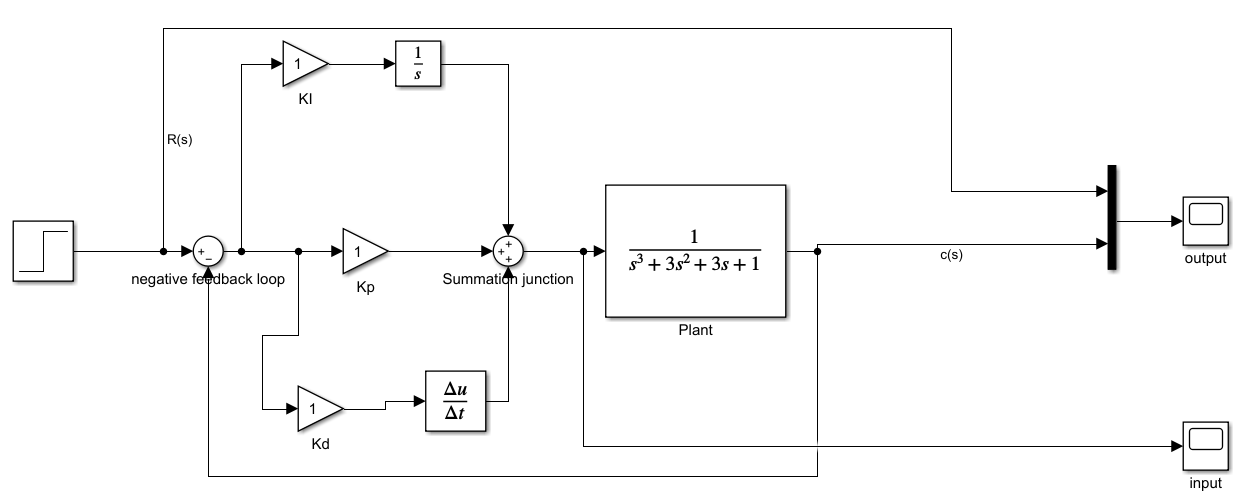
\includegraphics[width=1.0\textwidth]{pidDiagram}
	\caption[PID Control Block Diagram]{Block diagram of a closed loop PID controller \cite{documentationsimulation}. The first block on the left is a step function set to 1. The three triangular blocks (from top to bottom) are the integral gain, proportional gain, and derivative gain terms. Each gain term is applied to its associated function and then summed together. The value produced is fed to the plant, which sends the signal back to the initial junction, and the result of each iteration is displayed to the output block.}
	\label{fig:pidDiagram}
\end{figure}
\section{Proportional Control}
A P-only controller takes the error and finds a proportion $k_c$ of it known as the controller gain. This type of controller is represented in the time domain by
\begin{equation}\label{eq:pterm}
u(t) =  k_c e(t) + u_b \quad .
\end{equation}
$U(t)$ represents the actual value of the controller output and $u_b$ represents the bias (the percentage of controller output that should produce a steady state). The bias is often set to 50\% controller output, but it is not required to be. Note that the controller gain must be of the correct sign to avoid making the process worse. By convention, (+) is a reverse acting controller (a controller whose output tends to increase as the measurement signal increases), and (-) is a direct acting controller (a controller whose output tends to decrease as the measurement signal increases). In the Laplace domain, p-only control is represented as a zeroth order function\footnote{Recall the Laplace transform $G(s) = \mathscr{L}\{g(t)\}$; for linear functions, $af(t) = aF(s)$} \cite{wang2020pid}.
\begin{equation}
\frac{U(s)}{E(s)} = k_p \quad\footnote{Note that $k_c = k_p$}
\end{equation}
where $U(s)$ is the control signal and $E(s)$ is the error . The main advantage of a p-only control is that it is fast responding. This is useful for UAVs that take on more acrobatic maneuvers. The main issue with using this type of control is that there is always going to be an offset, that is, the process will never reach the desired steady state \cite{aastrom2006advanced}. As $k_c$ is increased, the system will get closer to its steady state, however, this also results in an increased likelihood in oscillations that lead to stability issues; see figure \ref{fig:pOnlyControl}.
\begin{figure}[H]
	\centering
	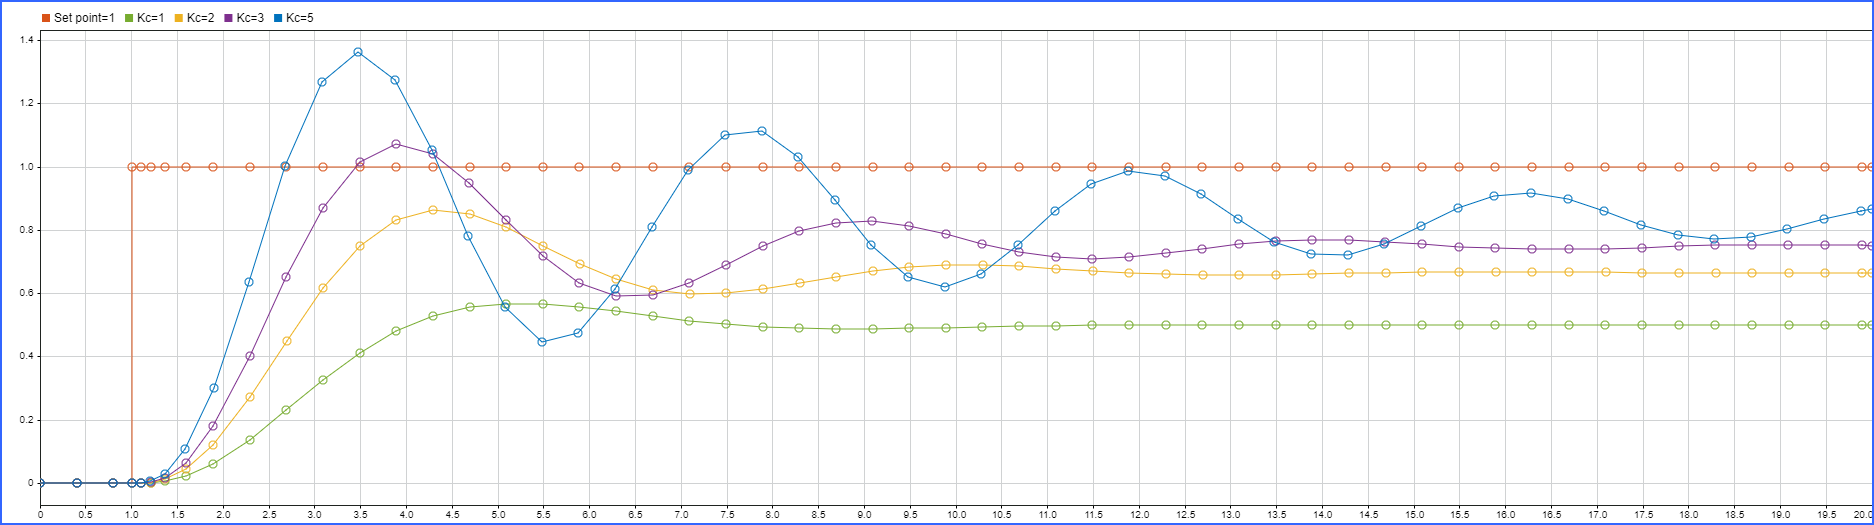
\includegraphics[width=1.0\textwidth]{pOnlyControl}
	\caption[P-only controller]{P-only controller for different values of $k_c$ and a transfer function of $G(s)=(1+s)^{-3}$. Note that as $k_c$ is increased, the system converges to the desired set point along with an increase in oscillations.}
	\label{fig:pOnlyControl}
\end{figure}
\section{Integral Control}
Pure I-control responds to the error by taking the integral of it and is represented as 
\begin{equation}
u(t) = K_c[e(t) + \frac{1}{\tau_I}\int_{0}^{t}e(t)dt]
\end{equation}
where $\tau_I$ is known as the reset time. The primary function of the integral action is to ensure that the process output agrees with the set point in steady state. This provides an alternative to the use of a control bias $u_b$ in Eq.\ref{eq:pterm}. The control bias is typically adjusted manually and requires exact knowledge of the process dynamics, which is not usually the case, so integral control is the preferred method \cite{aastrom2010feedback}. This guarantees that the system will eventually reach zero error by eliminating the offset. With integral action, a small positive error will lead to an increased control error and a negative error will give a decreased control signal \cite{aastrom2006advanced}. In the Laplace domain, the transfer function is\footnote{The Laplace transform of an integral is $\mathscr{L} \{\int_{0}^{t}g(t)dt\} = \frac{G(s)}{s}$.}
\begin{equation}
\frac{U(s)}{E(s)} = \frac{k_I}{ s}\quad\footnote{The integral gain $k_I = \frac{k_c}{\tau_I}$.}
\end{equation}
where $k_I$ is the integral gain constant. Although the integral control is beneficial in removing the offset, it is much more susceptible to stability issues and is therefore rarely used as a stand alone control \cite{patrick2009industrial}. It is also incapable in handling sustained error because the controller will saturate causing control of the system to be lost. This is know as integrator windup and is typically caused by limitations in the actuators; for example a valve cannot be more than fully opened or closed.
\begin{figure}[H]
	\centering
	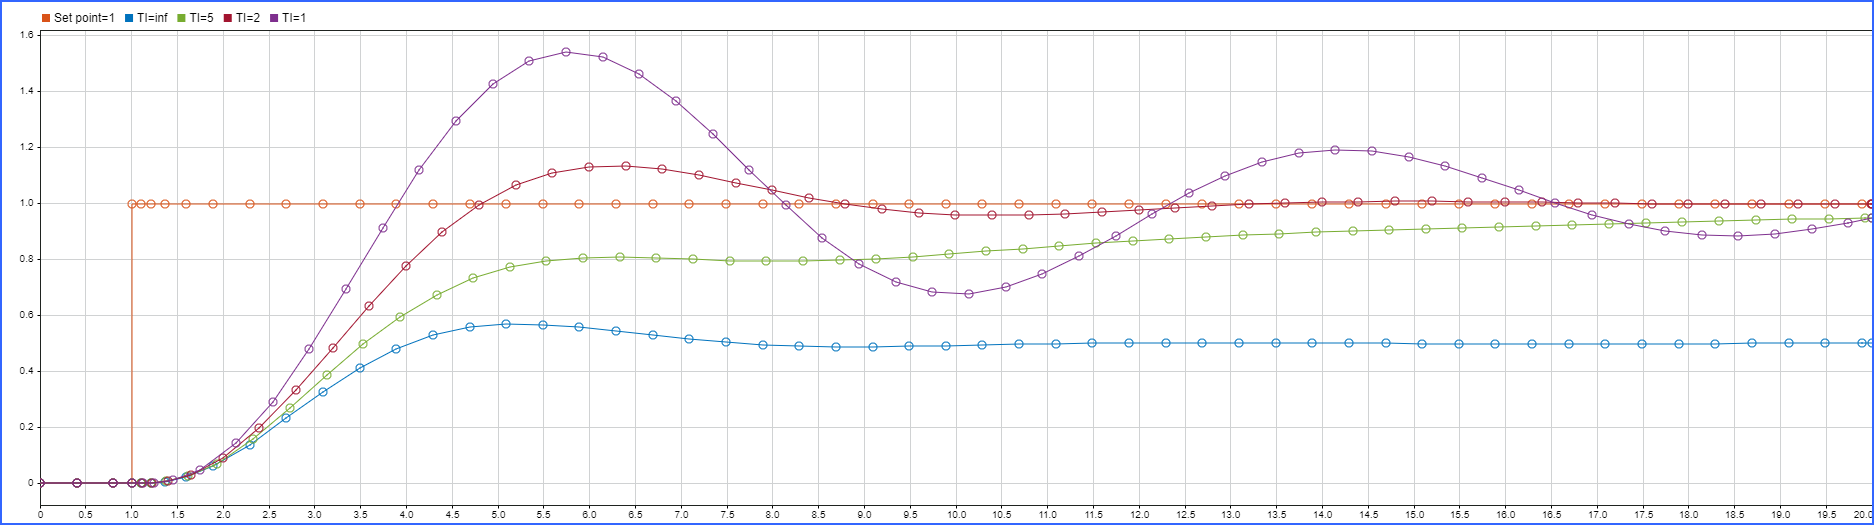
\includegraphics[width=1.0\textwidth]{IcontrolPat1}
	\label{fig:IOnlyControl}
	\caption[PI-controller]{PI-controller for different values of $\tau_I$. A transfer function of $G(s)=(1+s)^{-3}$ is used with the proportional gain held constant at 1. $\tau_I = \infty$ corresponds to pure proportional control and the system converges to the steady state error of 50\%. When $\tau_I$ is finite, the error is removed and the response moves toward the set point as $\tau_I$ is increased.}
\end{figure}
\section{Derivative Control}
The main function of the derivative action is to improve the stability of the closed loop \cite{wang2020pid}. This type of control is most useful when process response is very slowly and is represented as
\begin{equation}\label{eq:deriv}
u(t) = K_c[e(t) + \tau_D\frac{de(t)}{dt}] \quad.
\end{equation}
Eq \ref{eq:deriv} can be interpreted as a predictive action. Considering the process dynamics, it takes time for a change in the control variable to produce a noticeable change in the process output. This means that the control system will be late to respond to an error. The predictive nature of the derivative control corresponds to exploiting the error of the tangent to the error of the curve itself. In the Laplace domain, we have
\begin{equation}
\frac{U(s)}{E(s)} = \tau_D s \quad\footnote{The Laplace transform of a derivative is $\mathscr{L} \{ \frac{dg(t)}{dt} \} = sG(s) - f(0^+)$}
\end{equation}
\begin{figure}[H]
	\centering
	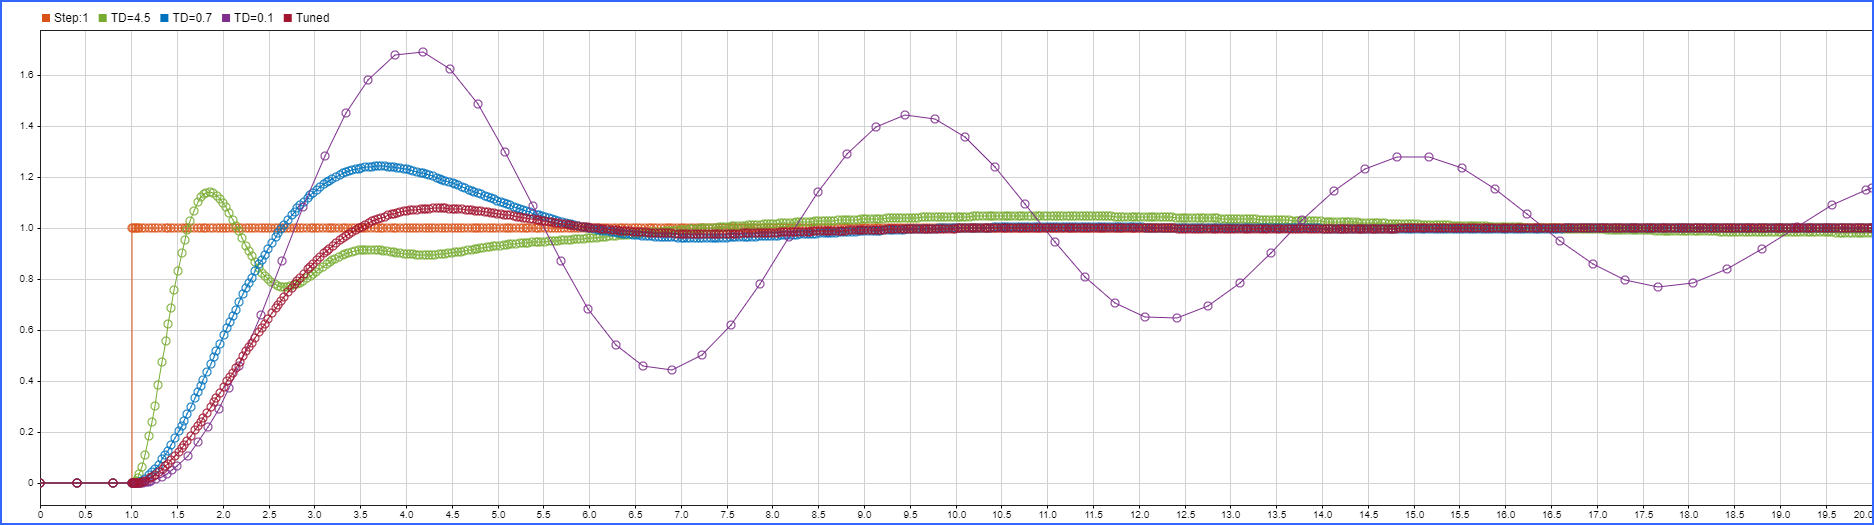
\includegraphics[width=1.0\textwidth]{tdSmall}
	\caption[PID-controller]{PID-controller with varying values of derivative time $\tau_d$ and a transfer function of $G(s)=(1+s)^{-3}$. The proportional gain is held at 3, while the reset time is held at 2. Note that the red line corresponds to a software tunning and PID values of $K_c=2.17$, $\tau_I=2.54$, and $\tau_D=0.55$.}
	\label{fig:td}
\end{figure}
\noindent
Because a larger $\tau_D$ corresponds to a faster the response, it is often referred to as the rate time, but it does not come without issues. High derivative control typically produces noisy data as can be seen more clearly using the Simulink scope, figure \ref{fig:dCompare}
\begin{figure}[H]
	\centering
	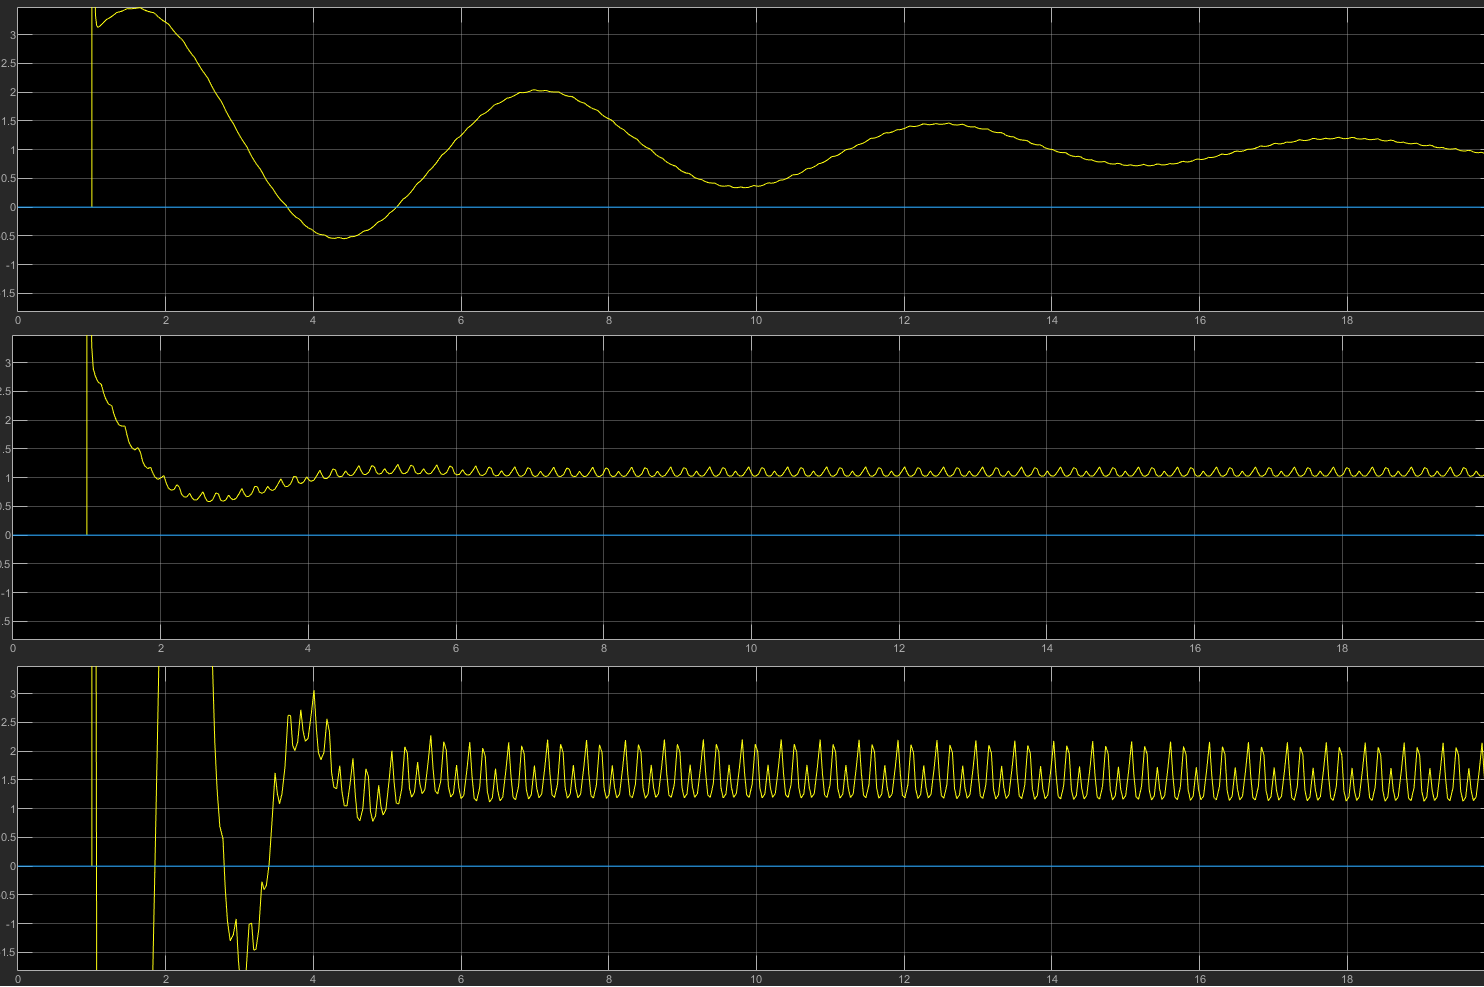
\includegraphics[width=12cm]{tdCompare}
	\caption[Noise fluctuations of derivative time]{Simulink scope view of derivative time \cite{documentationsimulation}. As the derivative time is increased, there is a corresponding increase in the noise of the measurement. From top to bottom, the derivate times are $\tau_D=0.1$, $\tau_D=0.7$,and  $\tau_D=4.5$.}
	\label{fig:dCompare}
\end{figure}
\noindent
With all terms considered, the full equation representing the output $U(t)$ of the PID controller in a closed loop system is, in the time domain
\begin{equation}
u(t) = K_c[e(t) + \frac{1}{\tau_I} \int e(t)dt + \tau_D \frac{de(t)}{dt}]
\end{equation}
and in the Laplace domain
\begin{equation}\label{eq:laplacefunction}
G(s) = K_p +\frac{K_I}{s} + K_Ds
\end{equation}
where $K_p = k_c$, $K_I = \frac{K_p}{\tau_I}$ and $K_d = K_p  \tau_d$.
\chapter{PID Controller Theory Applied to a UAV}
\section{Experimental Setup}
\begin{figure}[H]
	\centering
	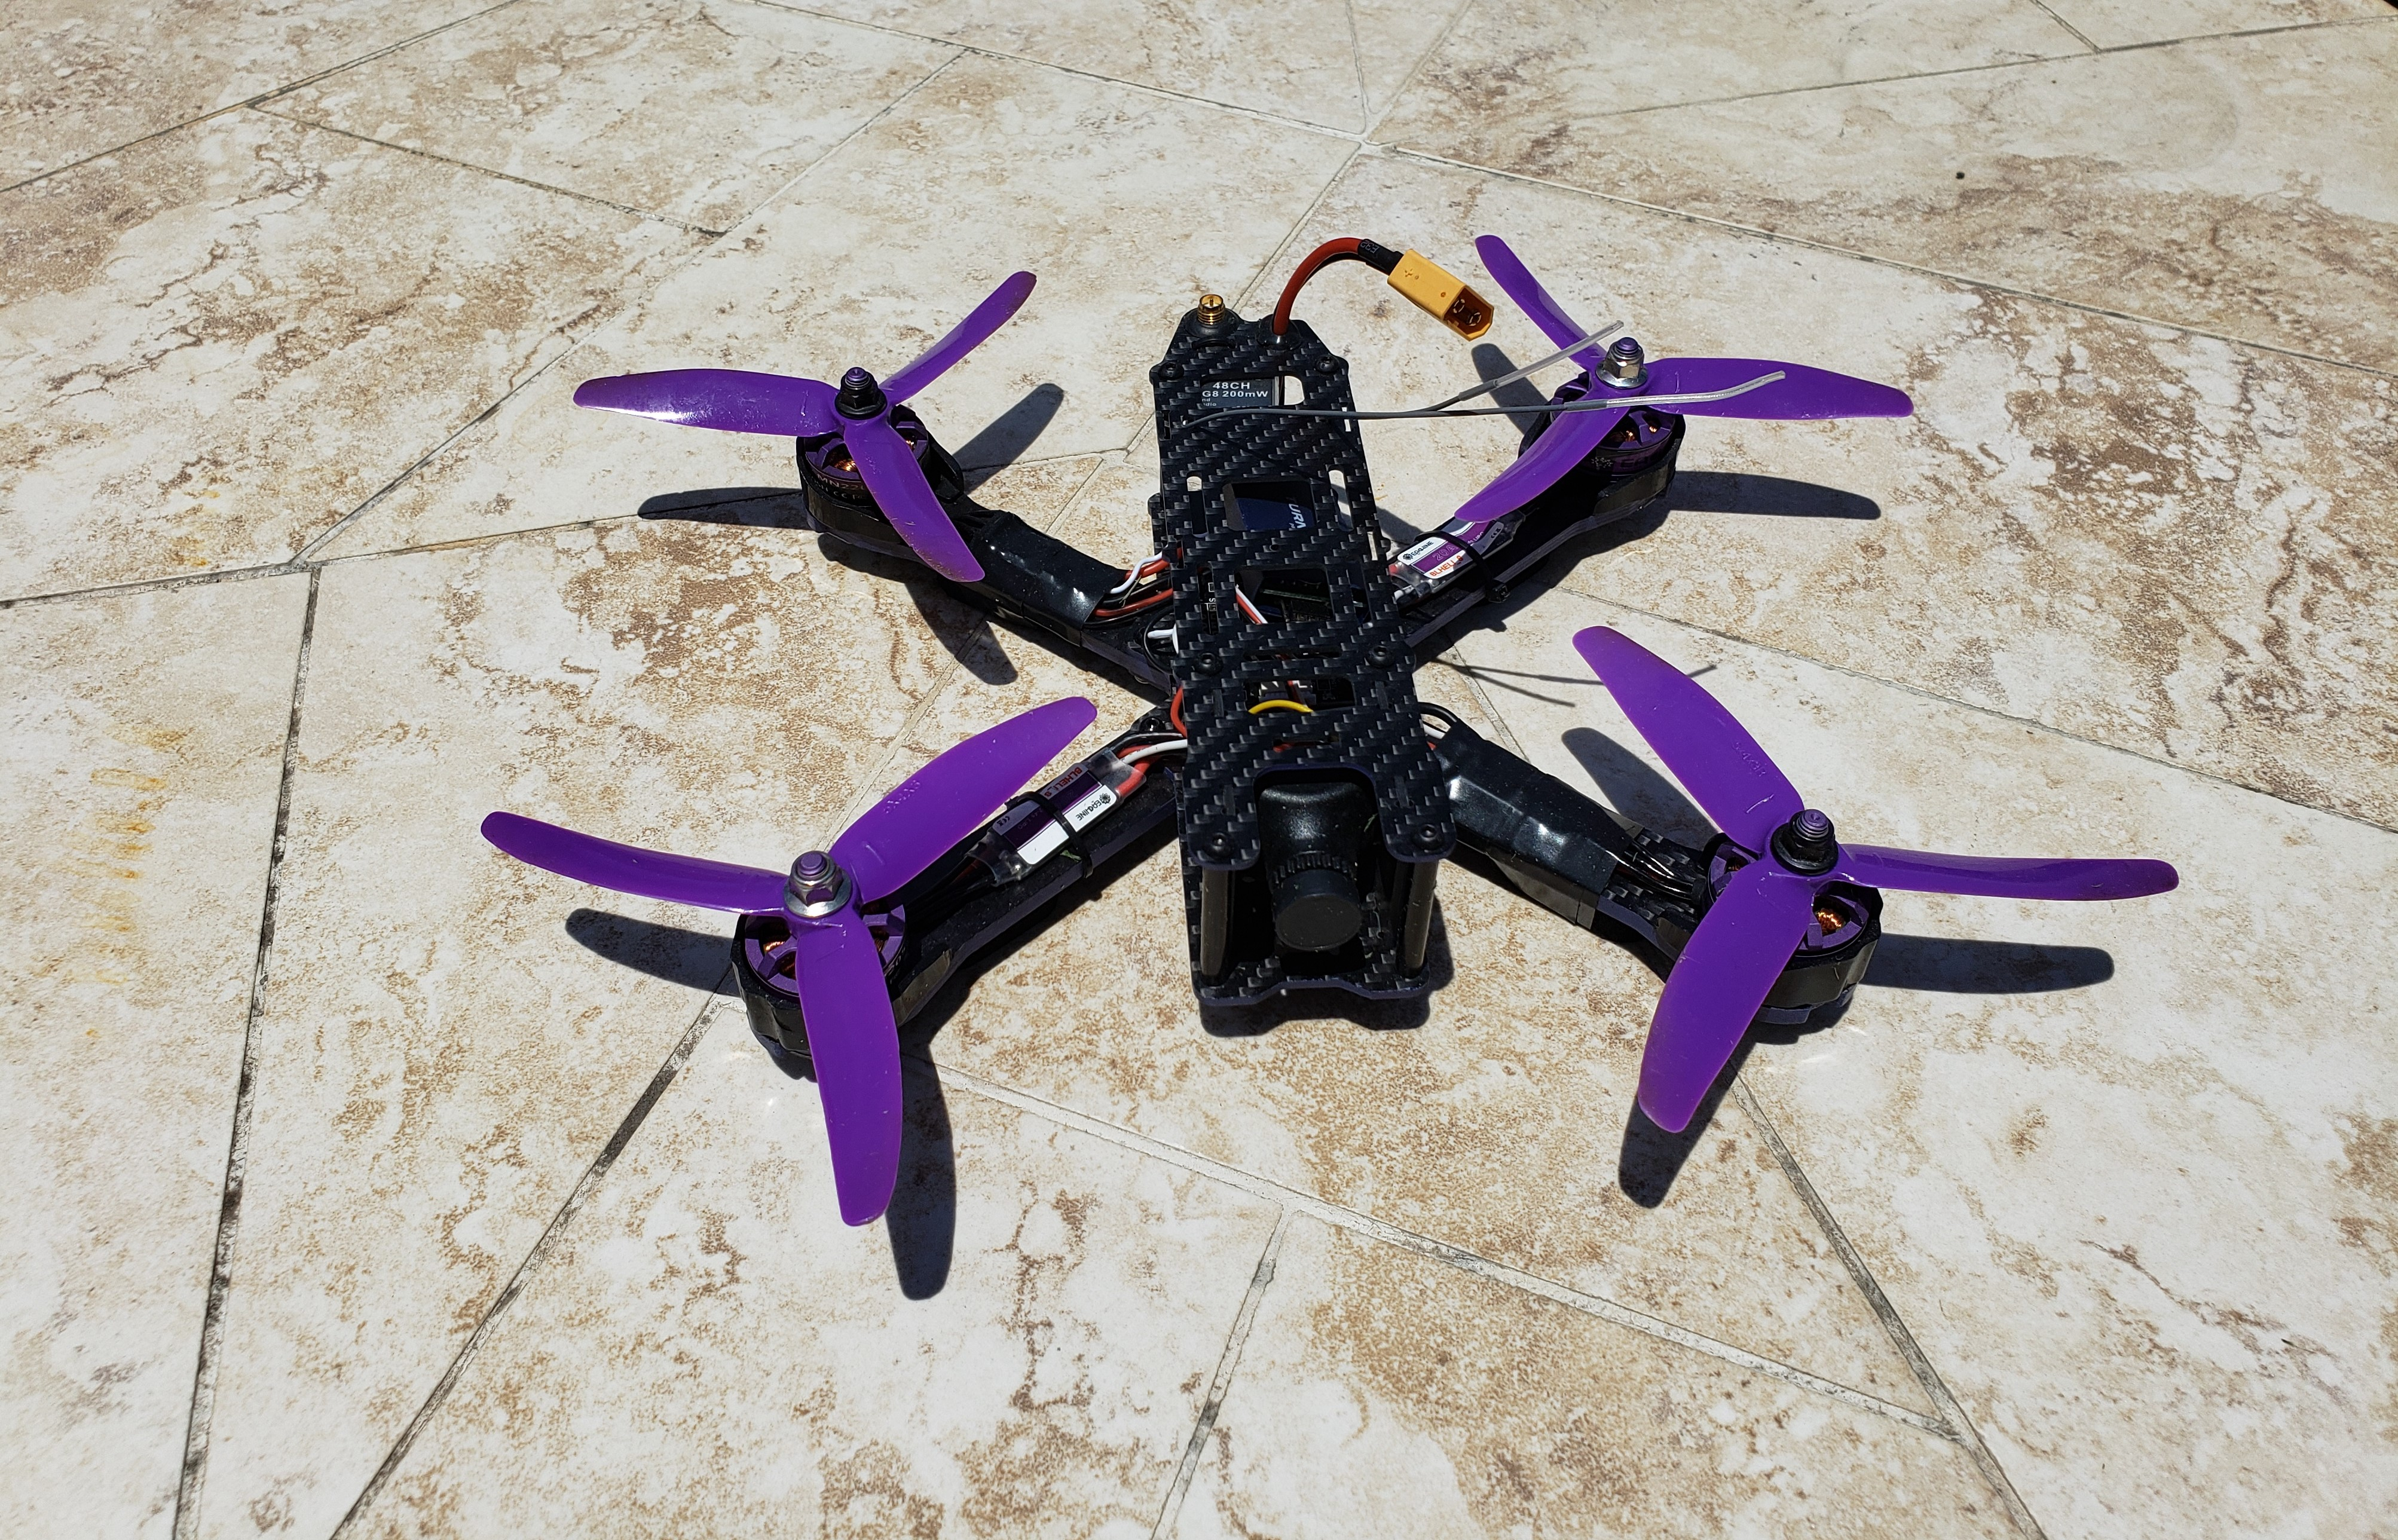
\includegraphics[width=\textwidth]{20200530_121423crop}
	\caption[Quadcopter]{Quadcopter used for pid analysis.}
	\label{fig:wizard1}
\end{figure}

All testing was performed using a 25.4 cm frame (diagonal measurement) in the X-configuration with 12.7 cm propellers in a triblade configuration. The electronic speed controllers are mounted to the middle of each arm and serve as regulators for the motors as shown in figure \ref{fig:wizard1} and figure \ref{fig:wizard2}. A 2.8mm 700TVL 1/3 CMOS camera is mounted to the front of the body and a video transmitter mounted at the rear. The entire system is powered by a 1300mAh, 65C rating, 4 cell lipo battery. The specifications of the motors and ESCs can be found in tables \ref{tab:Motors and ESC Specifications} and \ref{tab:Transmitter and receiver specifications}. The data were collected via a SP Racing F3 Flight Controller mounted to the center of the craft as shown in figure \ref{fig:wizard2}, the schematics of which can be found in figure \ref{fig:sp_racing_pro_f3}. The entire system was controlled using a 10 channel transmitter as shown in figure \ref{fig:transmitter}.
\begin{figure}[H]
	\centering
	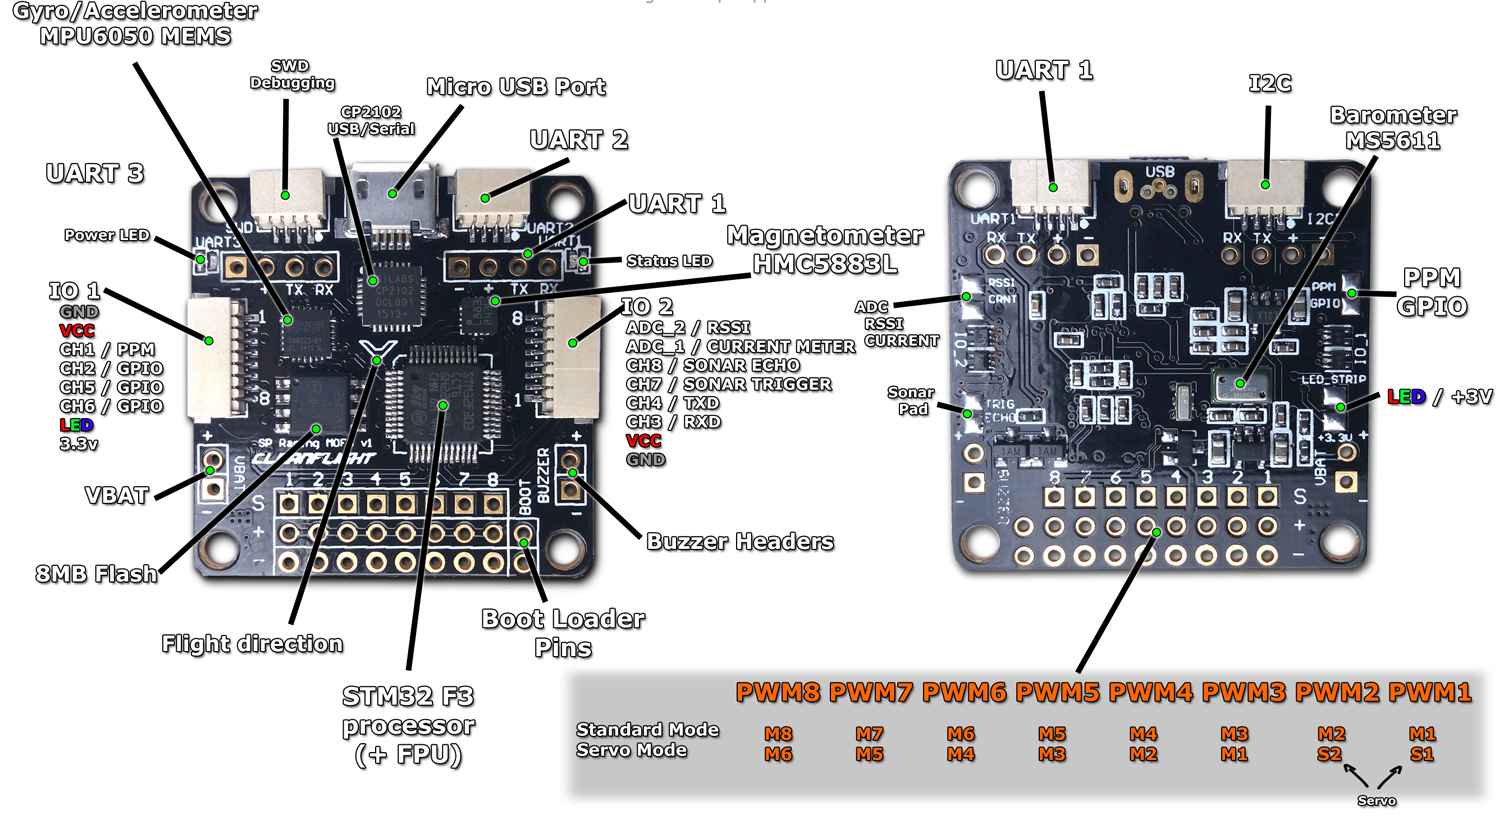
\includegraphics[width=\textwidth]{sp_racing_pro_f3}
	\caption[SP Racing F3 Flight Controller pin configuration]{SP Racing F3 Flight Controller pin configuration \cite{flightcontroller}. The flight controller acts as the brain of the copter. Its function is to take remote user input to control the speed of the motors and make the system move as instructed. The circuit board has a range of sensors incorporated into it including a gyro and accelerometer. There are 64mbs of storage to accommodate the flight controller software with approximately 8mb left over to collect data.}
	\label{fig:sp_racing_pro_f3}
\end{figure}
\noindent
The user can input stick commands that are transmitted to a receiver connected to the flight controller. In figure \ref{fig:transmitter}, The left stick is programmed to act as a throttle and yaw command, while the right sticks serves pitch and roll commands. The copter is armed with a toggle switch on the top of the transmitter. 
\begin{figure}[H]
	\centering
	
\includegraphics[width=\textwidth,height=\textheight,keepaspectratio]{flysky2}
	\caption[Transmitter]{Flysky FS- i6 radio transmitter \cite{transmitter}. The transmitter is used by the pilot to send commands to the flight controller. This particular model operates at a 2.4GHz frequency and has a range of 1500 meters. 10 channels are available to program by the user.}
	\label{fig:transmitter}
\end{figure}
\section{Tuning}
Any controller system straight out of the box requires a calibration. The exact weight of each quadcopter varies depending on the materials used, the amount of hardware connected to it, the size of the propellers etc. So it is not feasible to assign universal PID gain values that produce a stable system for every individual setup. Also, it is often the case that different copters should behave differently in various situations, but an ideal behavior for a quadcopter could be to exhibit minimal oscillations as it descends. For example, figure \ref{fig:initread} shows the PID response of the flight controller as the copter descends to the ground with default PID values assigned by the Betaflight software. It is clear that the copter exhibits excessive amounts of oscillation.
\begin{figure}[H]
	\includegraphics[width=1\textwidth]{initialreading}
	\caption[Preliminary PID Reading]{Preliminary PID response using default PID gain values of the flight control software. Note that yaw $\psi$, pitch $\theta$ and roll $\phi$ each have their own PID values assigned to them. The yaw response shows no measurement because only pitch and roll were used to land the copter.}
	\label{fig:initread}
\end{figure}
\subsection{Ziegler-Nichols’ Method}
In an ideal scenario, a PID tuning procedure would consist of an automatic software tune where the optimal PID values are determined by modeling a plant transfer function after input/output data as shown in figure \ref{fig:td}. This offers the most accurate gain values to produce a stable system or to achieve a desired behavior. However, it is not uncommon that the exact form of the plant transfer function is unknown. In this case, a heuristic method of PID tuning is appropriate. This is an acceptable approach to controller tuning because the PID controller has so few parameters. The method used to tune this specific quadcopter is based off the Ziegler-Nichols’ method \cite{aastrom2010feedback}. It was first developed in the 1940s and consists of setting the Integral time $\tau_I$ to infinity and derivative time $\tau_d$ to zero while the proportional gain $k_c$ is increased until stable oscillations occur. The maximum value of $k_c$ that produces stable oscillations is referred to as the ultimate gain $k_u$, and the frequency of the oscillation is known as the ultimate period $P_u$ \cite{wang2020pid}. Once the ultimate gain is determined, the integral gain is increased until the system exhibits a divergent oscillation, at which point the integral gain is dialed back slightly and the derivative gain is increased until the system stabilizes. The 1942 Ziegler-Nichols’ paper \cite{ziegler1942optimum} was written to provide optimal PID value ratios that could be used as a starting point for manually adjusting a controller. The results of the paper are summarized in table \ref{tab:Ziegler-Nichols’ control parameters}. This is extremely useful considering that manual tuning is a time consuming process. 
\begin{table}[H]
	\begin{center}
		\begin{tabular}{ |c|c|c|c| } 
			\hline
			Controller & $k_c$ & $\tau_I$ &  $\tau_d$ \\
			\hline
			P & 0.5$k_u$ & $\infty$ & 0\\ 
			PI & 0.45$k_u$ & 0.8 $p_u$ & 0\\ 
		 	PID & 0.6$k_u$ & 0.5 $p_u$ & 0.13 $p_u$\\ 
			\hline	
		\end{tabular}
	\caption{Ziegler-Nichols’ control parameters}
	\label{tab:Ziegler-Nichols’ control parameters}
	\end{center}
\end{table}
\subsection{Procedure}
With the Ziegler-Nichols’ control parameters in table \ref{tab:Ziegler-Nichols’ control parameters} in mind, the quadcopter was manually tuned. That is, for each of the three Euler angles $(\psi,\theta,\phi)$, one of the the PID gains is increased while holding the other two constant until minimal oscillations for that term are observed. For each run, the copter was brought to a static hover, then was allowed to yaw $360^\circ$ about the z-axis, pitch left and right, and finally roll forward and backward before allowed to descend. Between each test run, the copter's flight controller was connected to a computer via USB and the value of each term was adjusted using the Betaflight graphical interface shown in figure \ref{fig:pidSample}. The loop time of the flight controller was set to $2KHz$ and collected the data using on-board storage. Once the data was collected, the log file was imported to the computer for analysis. The log file was processed by PlasmaTree PID Analyzer which automatically generates graphs of the data.
\begin{figure}[H]
	\centering
	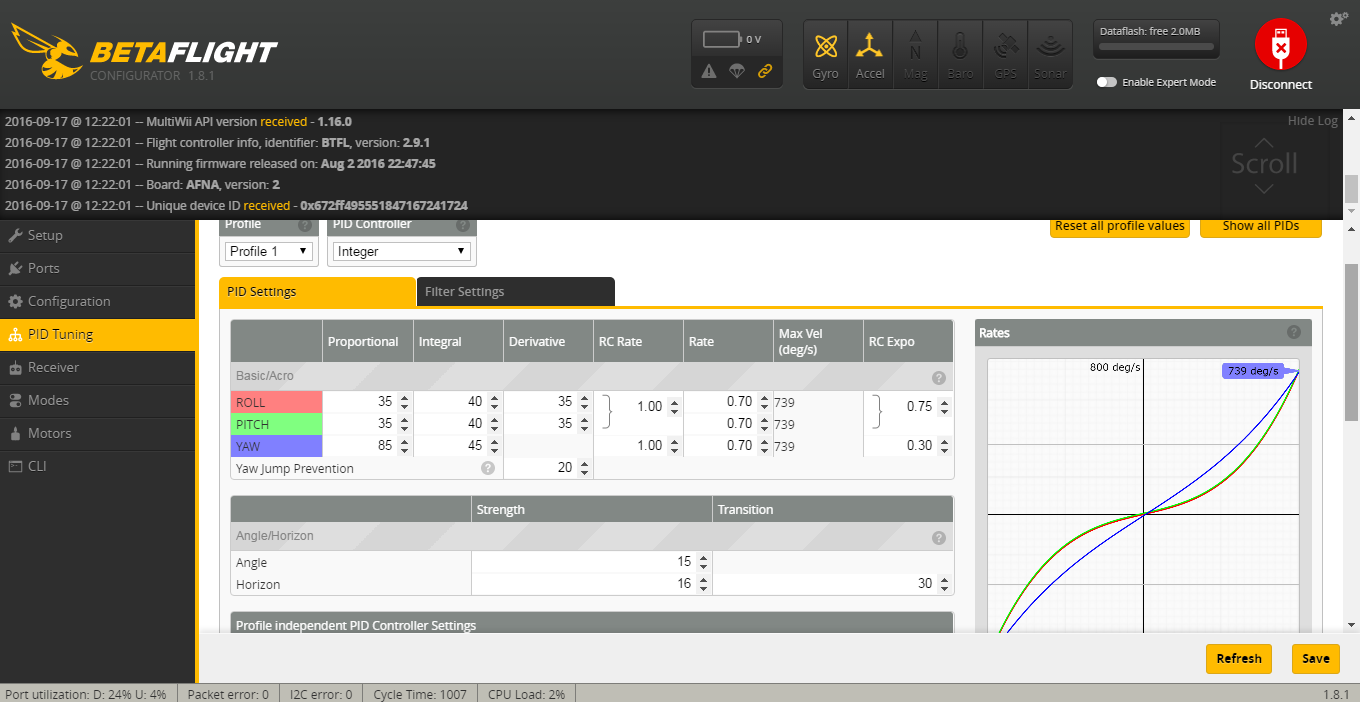
\includegraphics[width=\textwidth,height=\textheight,keepaspectratio]{pidSample}
	\caption[Betaflight PID configuration tool.]{Betaflight PID configuration tool. The proportional, integral and derivative terms for yaw, pitch and roll can be adjusted independent of each other. \cite{Betaflight}}
	\label{fig:pidSample}
\end{figure}
\section{Results}
 Figures \ref{fig:P_influence} - \ref{fig:D_influence} were created using PlasmaTree PID Analyzer \cite{plasmatree}, and the quadrotor was tuned manually. The copter was flown outside in a low wind environment. For each test run, yaw, pitch and roll were commands were sent to the flight controller via the transmitter in figure \ref{fig:transmitter}. The oscillations in pitch and roll were measured by holding the copter in hover and moving right stick of the transmitter in short quick bursts in all four directions (forward/backward and left/right). Between each movement, the stick was brought back to the center position until the copter returned to a stable hover. The response in yaw was measured by moving the left stick of the transmitter to the right in short quick movements until the copter completed a 360$^\circ$ turn about the z-axis of the body frame. The copter was then landed and disabled. Between each flight, a log file was extracted from the flight controller's black-box via USB, and was processed by the PID analyzer to produce a plot of the data, after which, the on-board storage of the flight controller was erased and the PID gains were increased for the next run. For each of the graphs in figure \ref{fig:P_influence} - \ref{fig:D_influence}, $t=0$ corresponds the the moment the input data is received. To analyze the effect of proportional control, $K_I$ and $K_D$ from Eq. \ref{eq:laplacefunction} were held constant at 10 units using the Betaflight GUI, while $K_p$ was allowed to vary from 10 units to 60 units for each of the three Euler angles. As can be seen from the plots in figure \ref{fig:P_influence}, increasing only the proportional gain to 60 units for yaw, pitch, and roll results in an overshoot to 1.5 for roll and pitch, followed by oscillations about the desired set point, while the yaw response undershoots and gradually approaches the set point. At this point, the oscillations observed had become apparent and the values were taken as an ultimate gain.
\begin{figure}[H]
	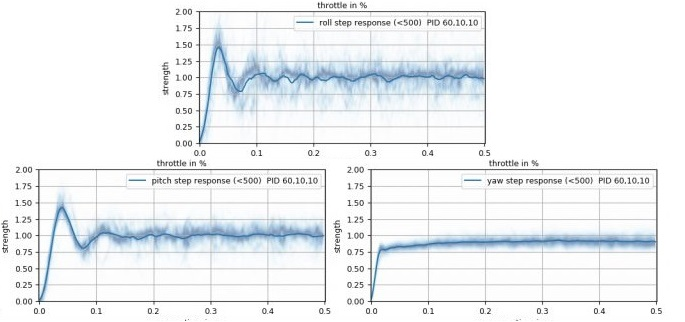
\includegraphics[width=1\textwidth]{P_influence}
	\caption[Proportion step response]{Proportion step response. }
	\label{fig:P_influence}
\end{figure}
\noindent
For the integral response tune, the derivative term was held at 10 units across the board and the proportional term was held at 70 units for yaw, 55 units for pitch, and 50 units for roll. By increasing the integral gain in 5 unit increments to 60 units, the offset in pitch, roll, and yaw approach the desired set point much faster, however as $K_I$ is increased, there is a corresponding increase in oscillation about the set point as shown in figure \ref{fig:I_influence}.
\begin{figure}[H]
	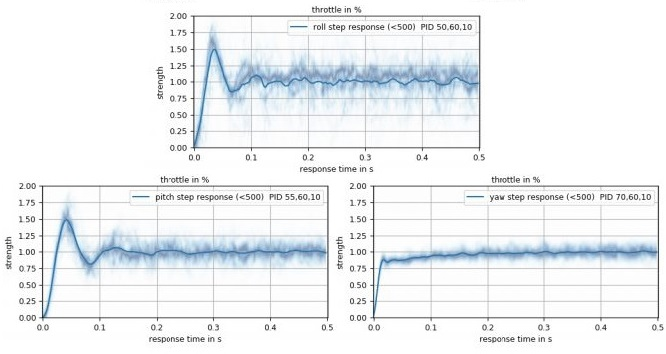
\includegraphics[width=1\textwidth]{I_influence}
	\caption[Integral step response]{Integral step response}
	\label{fig:I_influence}
\end{figure}
\noindent
Finally for the derivative response term, $k_p$ was held 50 units for roll, 55 units for pitch and 80 units for yaw, while $k_I$ was held at 45 units for roll, 55 units for pitch, and 60 units for yaw. The derivative term was allowed to progress in 5 unit increments until the oscillations were apparent during flight, and then dialed back. As the derivative term $K_d$ is increased, the overshoot exhibited in figure \ref{fig:P_influence} is rectified, and there is a significant reduction in noise produced by the throttle input. 
\begin{figure}[H]
	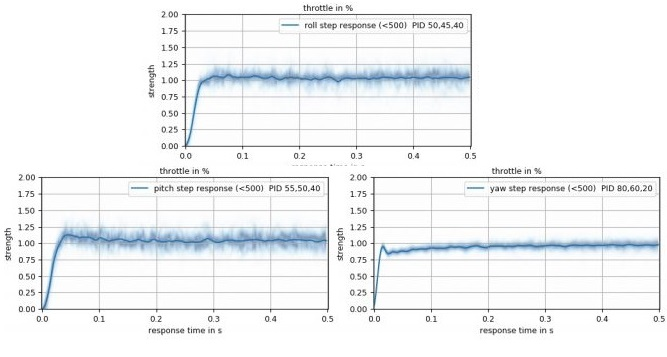
\includegraphics[width=1\textwidth]{D_influence}
	\caption[Derivative step response]{Derivative step response }
	\label{fig:D_influence}
\end{figure}
\noindent
By altering the PID gain values of the quadcopters flight controller, the response of the system is increased and stabilized. With a faster response time, the copter is able to maneuver more quickly and precisely with minimal oscillations and minimal deviations from the users input commands. This allows for a more predictable flight when the input is abrupt, or when external disturbances disrupt copters flight path. 


\nocite{*}
\bibliographystyle{plain}
\bibliography{uctest}
\appendix

\chapter{Appendix}
\vspace{-1cm}
\begin{figure}[H]
	\centering
	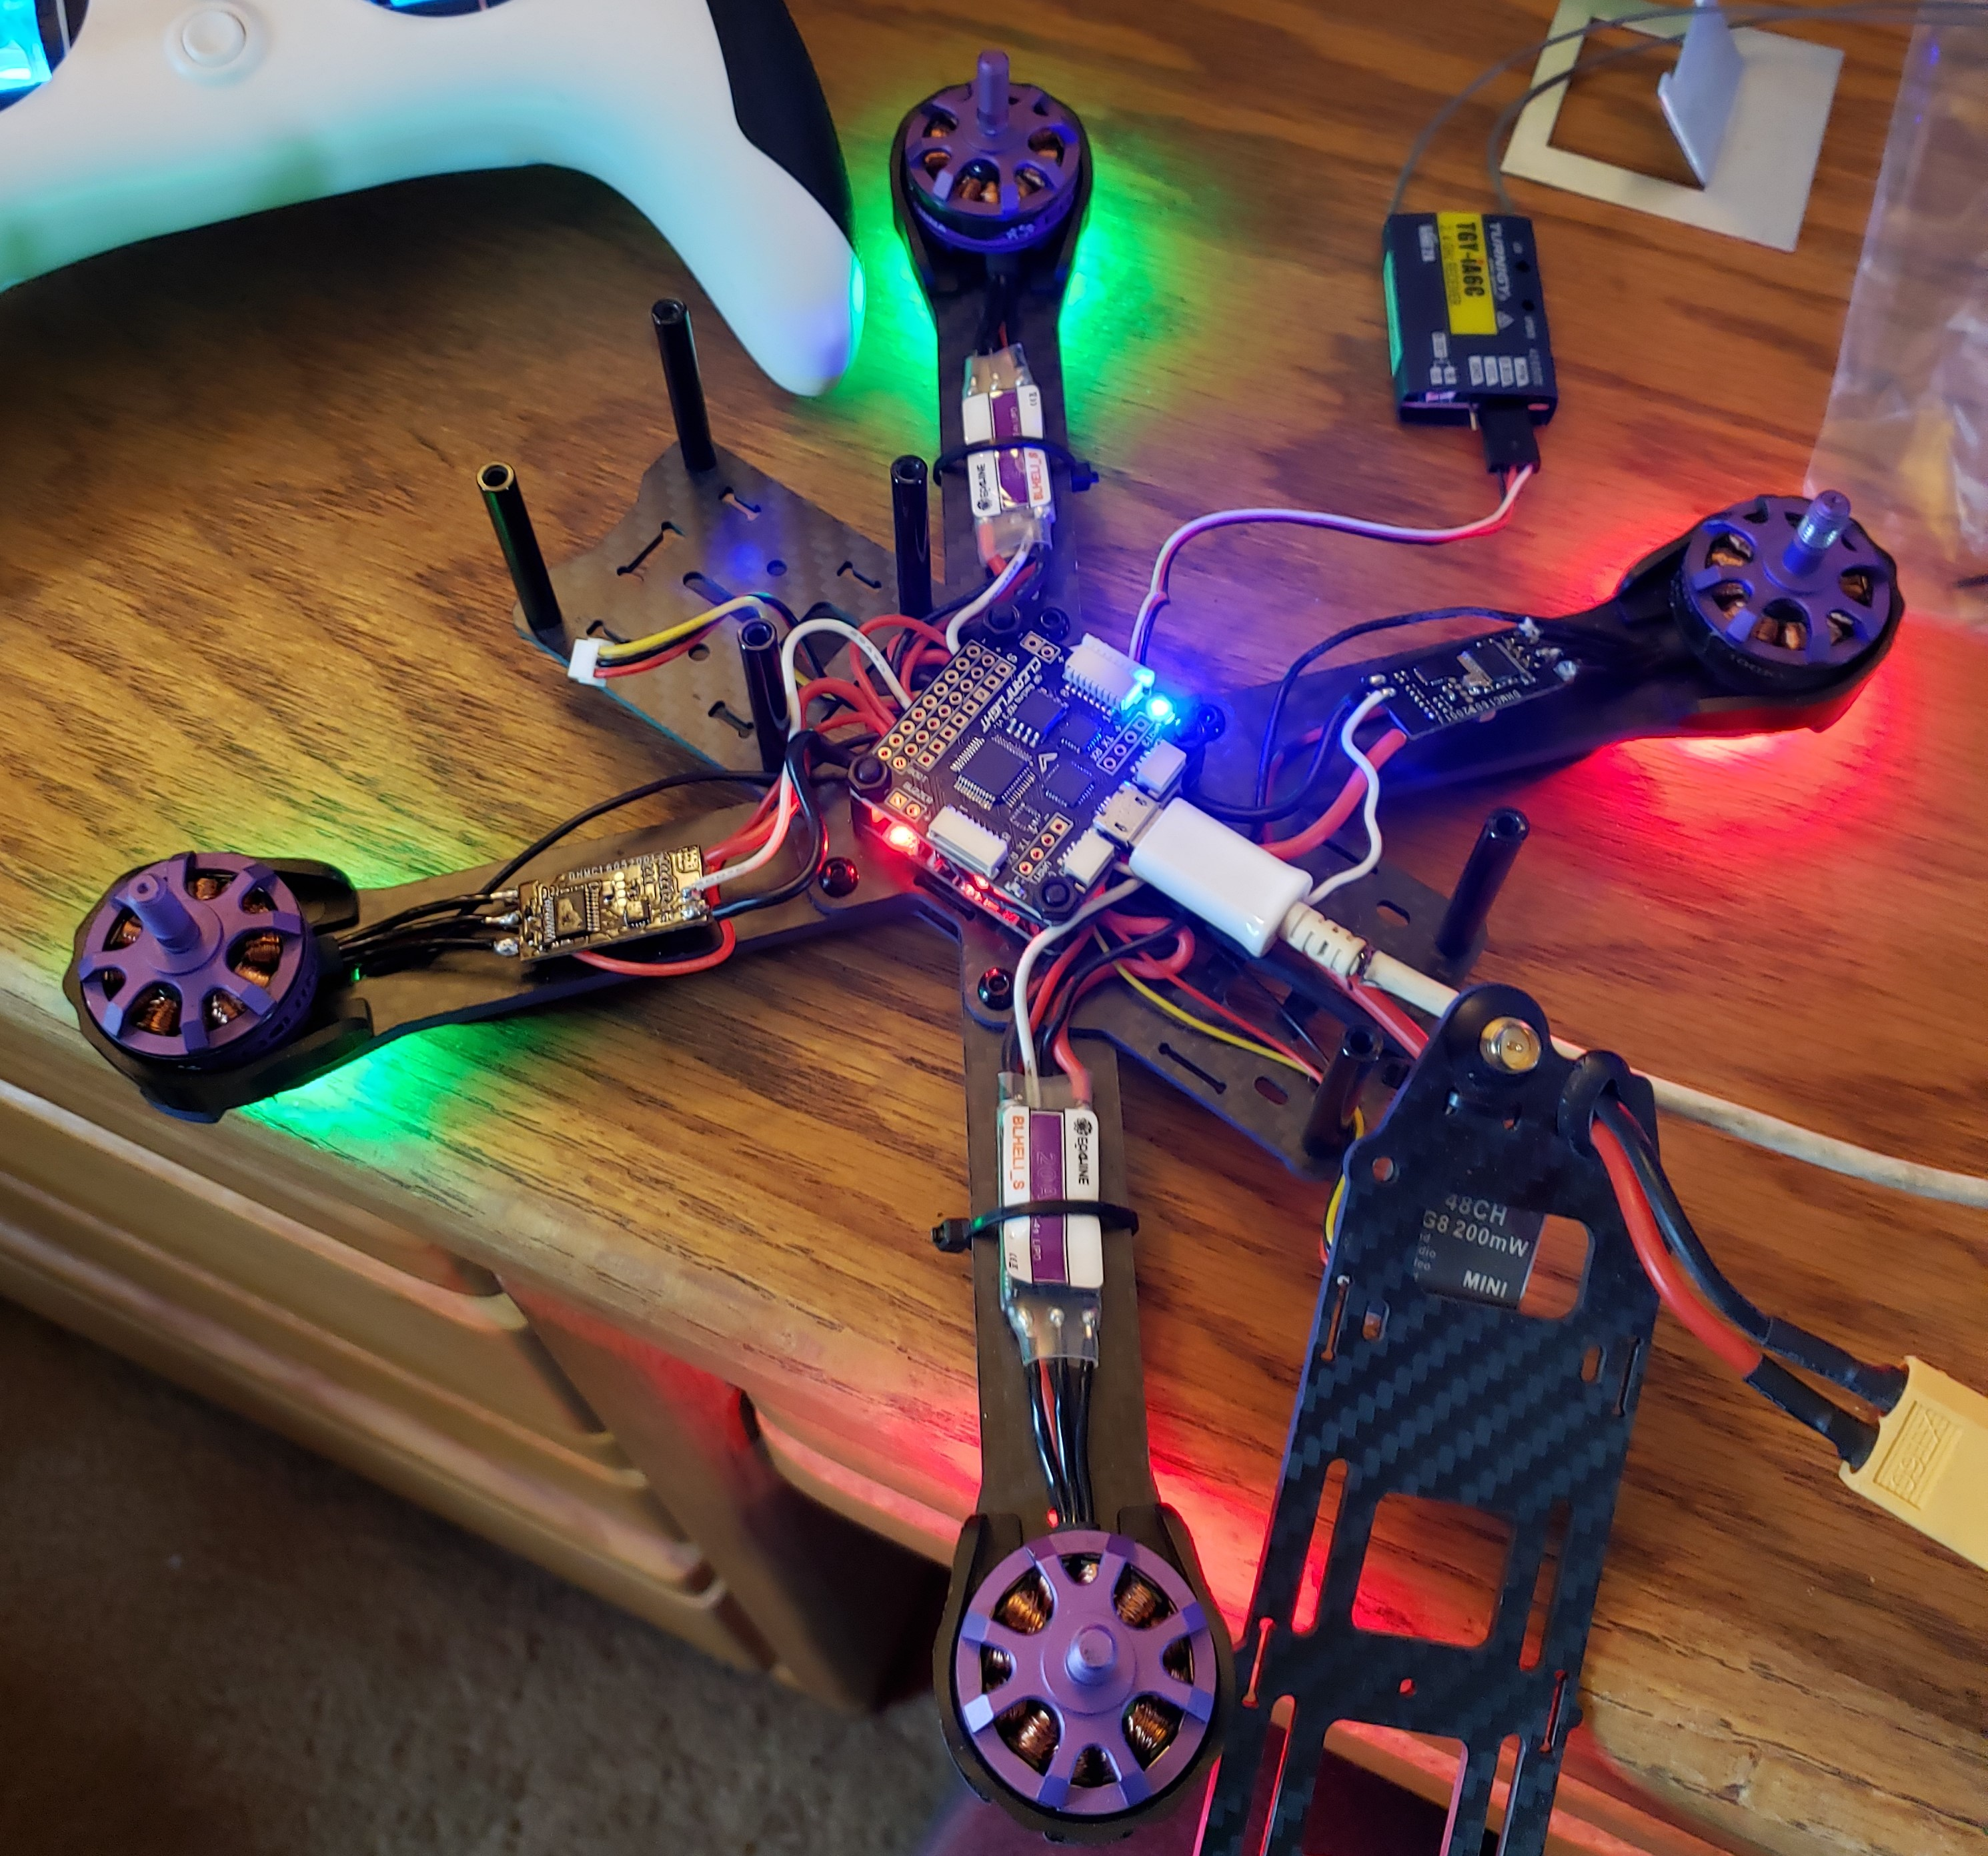
\includegraphics[width=0.75\textwidth]{20200322_154331crop}
	\caption[Internal Circuitry ]{The flight controller is mounted to the middle of the copter, with the electronic speed controllers soldered directly to it. The ESCs are mounted to each arm and soldered to MN2250 Brushless Motors. 5 volts of power is supplied to the circuit via a TRX connector. The system is controlled with a 2.4G receiver connected to the flight controller and mounted to the center of the craft with Velcro. Toward the front of the craft is space for a camera which is also connected to the flight controller.}
	\label{fig:wizard2}
\end{figure}
\vspace{3cm}
\begin{center}
	\begin{table}
		\caption{Motors and ESC Specifications}
		\begin{tabular}{|c|c|c|c|}
			\hline
			\multicolumn{2}{ |c| }{MN2250 Brushless Motors} \\\hline
			\hline
			kV&2300  \\
			\hline
			Max thrust&$\approx$ 780g  \\ 
			\hline
			Length&32.2mm\\
			\hline
			Input Voltage&7.4V-14.8V\\
			\hline
			Diameter&27.9mm\\
			\hline
			Configuration&12N14P\\
			\hline
			Shaft size(internal)&3mm\\
			\hline
			Prop size&12.7cm (max)\\
			\hline
			Weight&25g\\
			\hline
		\end{tabular}
		\quad
		\begin{tabular}{|c|c|c|c|}
			\hline
			\multicolumn{4}{ |c| }{MN2250 Brushless Motors} \\\hline
			\hline
			Current & 20A  \\
			\hline
			Peak current & 25 A  \\ 
			\hline
			Input Voltage &7.4-14.8V\\
			\hline
			Firmware & BLHeli s\\
			\hline
			PCB size & 27x12 mm\\
			\hline
		\end{tabular}
		\label{tab:Motors and ESC Specifications}
	\end{table}
\end{center}


\vspace{-1cm}
\begin{center}
	\begin{table}
		\caption{Transmitter and receiver specifications}
		\begin{tabular}{|c|c|c|c|}
			\hline 
			\multicolumn{2}{|c|}{FS-iAB6B Transmitter} \\\hline
			\hline
			Channels & 6  \\
			\hline
			Output Frequency & 2.40-2.48 GHz  \\ 
			\hline
			Bandwidth & 500 KHz\\
			\hline
			DSC port &PS2;Output:PPM\\
			\hline
			Antenna length  & 26mm * 2 dual\\
			\hline
			Power & 6V \\
			\hline
			Control range & 500 m\\
			\hline
			Weight & 25g\\
			\hline
		\end{tabular}
		\quad
		\begin{tabular}{|c|c|c|c|}
			\hline 
			\multicolumn{2}{ |c| }{FS-iAB6B Receiver} \\\hline
			\hline
			Channels & 6  \\
			\hline
			Bandwidth number & 140  \\ 
			\hline
			Transmitting power & $\leq$ 20 dBm\\
			\hline
			Encoding & GFSK \\
			\hline
			Antenna length  & 26mm * 2 dual\\
			\hline
			Input power & 4.0 - 6.5 V DC\\
			\hline
			Interface & i-BUS\\
			\hline
		\end{tabular}
	\label{tab:Transmitter and receiver specifications}
	\end{table}
\end{center}





\end{document}
